\documentclass{article}
\usepackage[utf8]{inputenc}
\usepackage{hyperref}
\usepackage[letterpaper, portrait, margin=1in]{geometry}
\usepackage{enumitem}
\usepackage{amsmath}
\usepackage{booktabs}
\usepackage{graphicx}
\usepackage{authblk}

\usepackage{hyperref}
\hypersetup{
colorlinks=true,
    linkcolor=black,
    filecolor=black,      
    urlcolor=blue,
    citecolor=black,
}
\usepackage{natbib}

\usepackage{titlesec}
  
\title{Homework Sample TeX Code}
\author{Kelly Lifchez}
\date{}
  
\begin{document}
  
\maketitle

\section{Introduction}

This sample TeX file can show you some tricks used to automatically update figures and tables.  This will get you started on the homework assignments if you are new to LaTeX.  Of course, Google is the best guide if you want to figure out how to do something.

\section{Nice math}
LaTeX allows you to format math equations easily and to align everything nicely.  For example, use the \verb! \begin{align}...\end{align}! environment with \verb!&! for column delimiters and \verb!\\! for row delimiters:

\begin{align}
    \hat{\beta}_{OLS} &= \text{arg}\min_{\beta} \sum_{i} (y_i - x_i \beta)^2 \\
    &= (X'X)^{-1}X'Y \label{eq:betahat}
\end{align}

\section{Sample mean table}
You can \textit{automatically} reference table and figure numbers using \verb!\label{}! and \verb!\ref{}!. See table \ref{tab:my_label}.

\subsection{Python version}

\begin{table}[ht]
    \centering
    \begin{tabular}{ll}
\toprule
 & Mean \\
 & (s.d.) \\
\midrule
Outcome & 206.51 \\
  & (43.91) \\
Variable 1 & 10.27 \\
  & (3.01) \\
Variable 2 & 20.22 \\
  & (3.80) \\
Observations & 100 \\
\bottomrule
\end{tabular}

    \caption{Sample mean table.  Make sure your captions are informative and that tables and figures can be understood out of context.}
    \label{tab:my_label}
\end{table}

\subsection{Stata version}

\begin{table}[ht]
    \centering
    {
\def\sym#1{\ifmmode^{#1}\else\(^{#1}\)\fi}
\begin{tabular}{l*{1}{c}}
\hline\hline
                    &\multicolumn{1}{c}{(1)}\\
                    &\multicolumn{1}{c}{}\\
                    &Mean/Std. Dev.\\
\hline
Variable 1          &       11.69\\
                    &     (10.36)\\
Variable 2          &       20.67\\
                    &     (14.46)\\
Outcome variable    &      209.30\\
                    &    (159.52)\\
\hline
Observations        &         100\\
\hline\hline
\end{tabular}
}

    \caption{Summary statistics produced using Stata}
    \label{tab:statasummary}
\end{table}

\section{Sample kernel density plot}
It is nice to center tables and figures.  When making figures, try to avoid using red and green colors together for accessibility.  See figure \ref{fig:samplehist}.

\subsection{Python version}

\begin{figure}[ht]
    \centering
    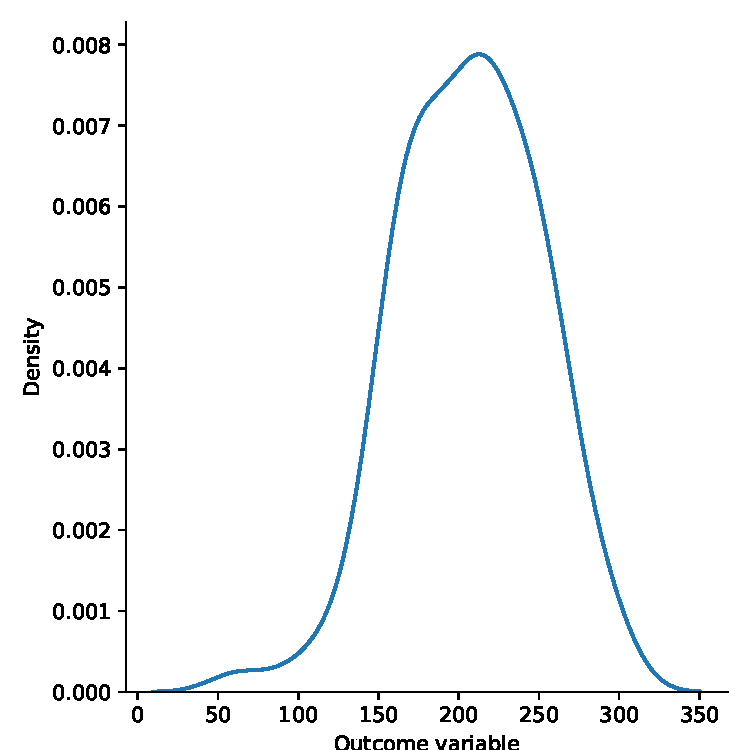
\includegraphics[scale = 0.7]{output/samplehist.pdf}
    \caption{Sample kernel density plot of the outcome variable.}
    \label{fig:samplehist}
\end{figure}

\subsection{Stata version}

Stata has a nice color scheme you can install that works for black and white printing and is color-blind accessible:

\begin{figure}[ht]
    \centering
    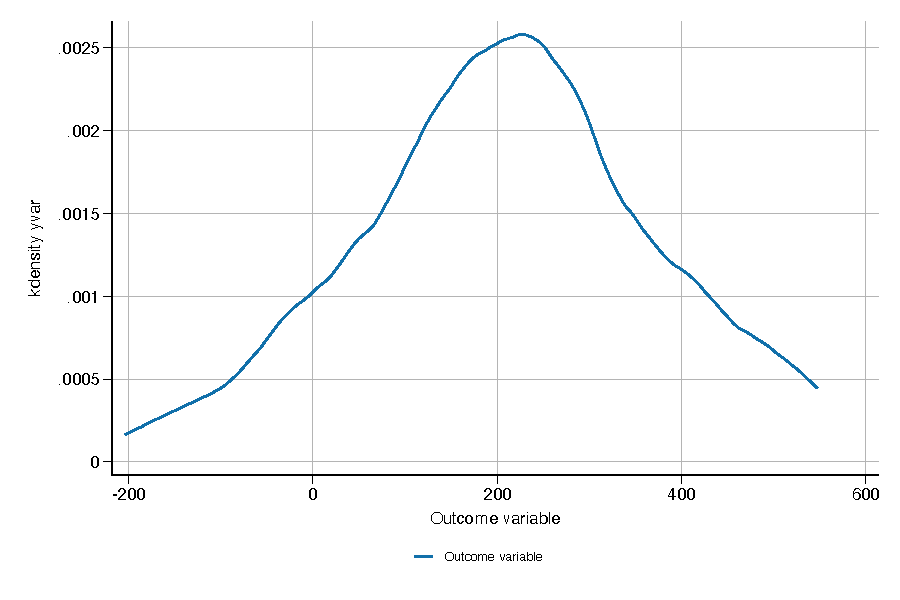
\includegraphics{output/statadensity.pdf}
    \caption{Sample kerndel density plot of the outcome variable generated in Stata}
    \label{fig:statahist}
\end{figure}

\section{Sample regression output with CIs}
You can see that tables can be updated and input into the main .tex file automatically.  To do this, you output your table to a separate .tex file and use \verb! \input{tablefilename.tex} ! to reference it.  This might seem silly, but when you have to estimate a dozen regressions over again because your advisor wants you to cluster your standard errors, you will save HOURS of formatting problems by automating.

\subsection{Python version}

See table \ref{tab:sampleoutput}:

\begin{table}[ht]
    \centering
    \begin{tabular}{ll}
\toprule
 & Estimates \\
\midrule
Variable 1 & -3.250000 \\
  & (-3.89, -2.75) \\
Variable 2 & 12.550000 \\
  & (12.09, 13.01) \\
Constant & -14.000000 \\
  & (-21.75, -6.99) \\
Observations & 100 \\
\bottomrule
\end{tabular}

    \caption{Sample regression output table with confidence intervals! Confidence intervals bootstrapped with 1000 replications.  One of the most important things to reference in a table caption is what standard errors you used.  It can also be useful to reference the estimating equation if that is in text. See equation \ref{eq:betahat} for the OLS estimator.}
    \label{tab:sampleoutput}
\end{table}

\subsection{Stata version}

See table \ref{tab:regression_output}. 
\begin{table}[ht]
    \centering
    \begin{tabular}{lc} \hline
 & (1) \\
VARIABLES & Ordinary least squares \\ \hline
 &  \\
Variable 1 & -3.03** \\
 & (0.29) \\
Variable 2 & 10.88** \\
 & (0.21) \\
Constant & 19.82** \\
 & (6.14) \\
 &  \\
Observations & 100 \\
 R-squared & 0.97 \\ \hline
\multicolumn{2}{c}{ Standard errors in parentheses} \\
\multicolumn{2}{c}{ ** p$<$0.01, * p$<$0.05} \\
\end{tabular}

    \caption{Sample regression output table with standard errors bootstrapped with 1000 replications.}
    \label{tab:regression_output}
\end{table}

\section{Sample regression visualization with CI error bars}
I really like using confidence intervals to express uncertainty about the estimates \citep[see e.g.,][]{zm2009}.  As a rule, it is better to display your results as images rather than as tables, though this is not always feasible. See figure \ref{fig:samplebars} for an example of how you could choose to display OLS estimates with confidence intervals.

\subsection{Python version}

\begin{figure}[ht]
    \centering
    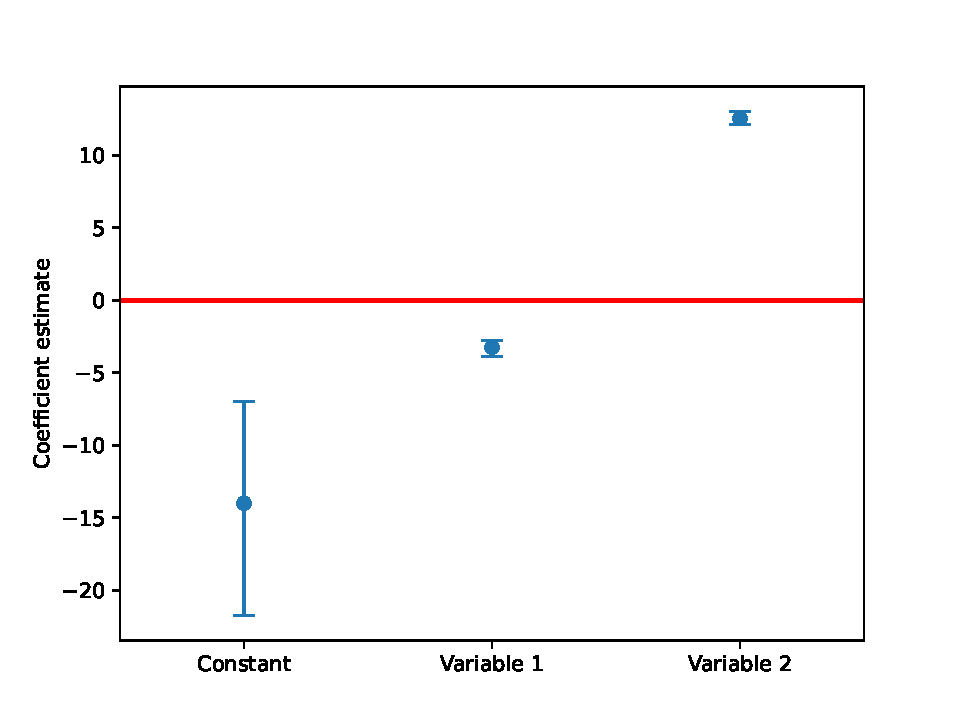
\includegraphics[scale = 0.7]{output/samplebars.pdf}
    \caption{Regression coefficient estimates with 95\% confidence intervals bootstrapped using 1,000 replications.}
    \label{fig:samplebars}
\end{figure}

\subsection{Stata version}

See figure \ref{fig:samplebars_stata}.
\begin{figure}[hb]
    \centering
    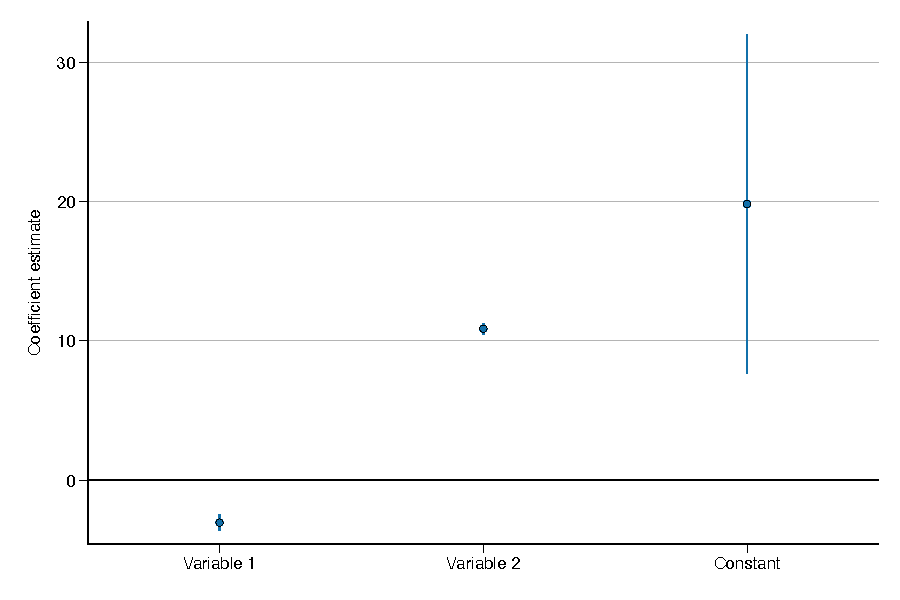
\includegraphics{output/samplebars_stata.pdf}
    \caption{Regression coefficient estimates with 95\% confidence intervals bootstrapped using 1,000 replications.}
    \label{fig:samplebars_stata}
\end{figure}

\section{You can also automate your bibliography}

You can include a bibtex/natbib bibliography that automatically formats your references, keeps them in order, and makes them into clickable hyperlinks. It's a little complicated to get started with, but this will also save you hours in the long run.  Imagining wasting time looking up Chicago, APA, or MLA formatting--this is a waste when you can automate it.

\section{Papers, slides, and other documents}
For research papers, it is probably best to use LaTeX for the reasons described above (especially when producing an empirical paper).  For presentations, many people use the Beamer theme of LaTeX.  I would recommend trying it out and keeping it for your job-market talk while in grad school, but in the long run I am less convinced it is worth it.  MS Powerpoint is much more customizable and is easier to fit tables on.  For other documents with less math and few tables/ figures, just use MS Word.

\bibliography{sampleref}
\bibliographystyle{chicago}

\end{document}